%%%%%%%%%%%%%%%%%%%%%%%%%%%%%%%%%%%%%%%%%%%%%%%%%%%%%%%%%%%%%%%%%%%%%%%%%%%%%%%%
% Preámbulo                                                                    %
%%%%%%%%%%%%%%%%%%%%%%%%%%%%%%%%%%%%%%%%%%%%%%%%%%%%%%%%%%%%%%%%%%%%%%%%%%%%%%%%

\documentclass[11pt,a4paper,titlepage,twoside,openright,openbib,spanish]{report}

%%% RELACIÓN DE VARIABLES A PERSONALIZAR %%%
\def\lingua{esp} % descomenta esta liña se redactarás a memoria en español
\def\nome{Alonso Rodríguez Iglesias}                             % substitúe aquí o teu nome
\def\nomedirectorA{Gabriel Rodríguez Álvarez}             % substitúe aquí o nome de quen dirixe
\def\nomedirectorB{Juan Touriño Domínguez}             % substitúe aquí o nome de quen dirixe
\def\titulo{Análisis del rendimiento de la inferencia de redes de aprendizaje profundo en arquitecturas de altas prestaciones} % substitúe aquí o título do teu TFM
% \def\mencion{ENXEÑARÍA DE COMPUTADORES}

\def\renomearcadros{si} % descomenta esta liña se redactas a memoria en español e prefires que
                         % os "cuadros" e o "índice de cuadros" se renomeen
                         % a "tablas" e "índice de tablas" respectivamente

\usepackage{estilo_tfm}

% Lista de paquetes potencialmente interesantes (uso baixo demanda)

\usepackage[all]{nowidow}
% \usepackage{alltt}       % proporciona o entorno alltt, semellante a verbatim pero que respecta comandos
% \usepackage{enumitem}    % permite personalizar os entornos de lista
% \usepackage{eurofont}    % proporciona o comando \euro
\usepackage{eurosym}
\usepackage{float}       % permite máis opcións para controlar obxectos flotantes (táboas, figuras)
\usepackage{hhline}      % permie personalizar as liñas horizontais en arrays e táboas
% \usepackage{longtable}   % permite construir táboas que ocupan máis dunha páxina
\usepackage{lscape}      % permite colocar partes do documento en orientación apaisada
% \usepackage{moreverb}    % permite personalizar o entorno verbatim
\usepackage{multirow}    % permite crear celdas que ocupan varias filas da mesma táboa
\usepackage{pdfpages}    % permite insertar ficheiros en PDF no documento
\usepackage{rotating}    % permite diferentes tipos de rotacións para figuras e táboas
% \usepackage{subcaption}  % permite a inclusión de varias subfiguras nunha figura
% \usepackage{tabu}        % permite táboas flexibles
% \usepackage{tabularx}    % permite táboas con columnas de anchura determinada
\usepackage{pdflscape}
\usepackage{translator}
\usepackage{placeins}
\usepackage{tablefootnote}

\usepackage[scale=MatchLowercase]{sourcecodepro}
\usepackage{pgfplots}
\usepackage{pgfgantt}
\newganttlinktype{F-S}{
  \ganttsetstartanchor{east}
  \ganttsetendanchor{west}
  \draw [/pgfgantt/link] (\xLeft - 0.2,\yUpper) -- (\xRight + 0.2, \yLower);
}

\newganttlinktype{F_S}{
  \ganttsetstartanchor{east}
  \ganttsetendanchor{west}
  \draw [/pgfgantt/link] (\xLeft - 0.2,\yUpper) |- (\xRight + 0.2, \yLower);
}

\newganttlinktype{S-S}{
  \ganttsetstartanchor{west}
  \ganttsetendanchor{west}
  \draw [/pgfgantt/link] (\xLeft + 0.2,\yUpper) |- (\xRight, \yLower);
}

\newganttlinktype{F-F}{
  \ganttsetstartanchor{east}
  \ganttsetendanchor{east}
  \draw [/pgfgantt/link] (\xLeft - 0.2 ,\yUpper) -| (\xRight - 0.2, \yLower);
}

\newganttlinktype{F-S}{
  \ganttsetstartanchor{east}
  \ganttsetendanchor{west}
  \draw [/pgfgantt/link] (\xLeft - 0.2,\yUpper) -| (\xRight + 0.2, \yLower);
}
\usepackage{pgfplotstable}
\pgfplotsset{compat = newest}
\usepackage{wrapfig}
\usepackage{etoolbox}
\BeforeBeginEnvironment{wrapfigure}{\setlength{\intextsep}{0pt}}
\usepackage{svg}
\usepackage{adjustbox}
\newcommand{\vasymptote}[2][]{
    \draw [thick,ficblue,densely dashed,#1] ({rel axis cs:0,0} -| {axis cs:#2,0}) -- ({rel axis cs:0,1} -| {axis cs:#2,0});
}
\pgfplotsset{every axis/.append style={
        scaled y ticks = false, 
        scaled x ticks = false, 
        y tick label style={/pgf/number format/.cd, fixed},
        x tick label style={/pgf/number format/.cd, fixed}
    }
}

%%%%%%%%%%%%%%%%%%%%%%%%%%%%%%%%%%%%%%%%%%%%%%%%%%%%%%%%%%%%%%%%%%%%%%%%%%%%%%%%
% Corpo                                                                        %
%%%%%%%%%%%%%%%%%%%%%%%%%%%%%%%%%%%%%%%%%%%%%%%%%%%%%%%%%%%%%%%%%%%%%%%%%%%%%%%%

\begin{document}

%%%%%%%%%%%%%%%%%%%%%%%%%%%%%%%%%%%%%%%%
% Preliminares do documento            %
%%%%%%%%%%%%%%%%%%%%%%%%%%%%%%%%%%%%%%%%

\begin{titlepage}
  
  \hspace*{128pt}
  \textcolor{udcgray}{{\fontencoding{T1}\fontfamily{phv}\selectfont Departamento de Ingeniería de Computadores}}\\[-2pt]
  \hspace*{145pt}
  \textcolor{udcpink}{{\fontencoding{T1}\fontfamily{phv}\selectfont Facultad de Informática de A Coruña}}\\[-32pt]

  \begin{center}
    
\includegraphics[scale=0.3]{img/udc.png}\\[35pt]

    {\large TRABAJO FIN DE MÁSTER \\
            MÁSTER INTERUNIVERSITARIO EN \\
            COMPUTACIÓN DE ALTAS PRESTACIONES } \\[100pt]
    
    \begin{huge}
      \begin{spacing}{1.3}
        \bfseries \titulo
      \end{spacing}
    \end{huge}
  \end{center}
  
  \vfill
  
  \begin{flushright}
    {\large
    \begin{tabular}{ll}
      {\bf Estudiante:} & \nome \\
      {\bf Directores:} & \nomedirectorA \\ % COPIA E PEGA ESTA LIÑA MÁIS VECES SE O PRECISAS
                        & \nomedirectorB \\ % COPIA E PEGA ESTA LIÑA MÁIS VECES SE O PRECISAS
    \end{tabular}}
  \end{flushright}
  \rightline{A Coruña, \today}
\end{titlepage}

\paxinaenbranco
\begin{flushright}
\dedicatoria{A todas las personas que me apoyaron en los buenos y los malos momentos.\\Gracias a ellos hoy soy quien soy.}
\end{flushright}
\paxinaenbranco
\paxinaenbranco
\begin{agradecementos}
A todas las personas que me han acompañado a lo largo de mi vida, en especial a mi familia y amigos, por estar ahí cuando se los necesitaba, por los buenos momentos que hemos pasado juntos, y su permanente e incondicional apoyo.

A todas las increíbles personas que he conocido y con las que he tenido el placer de compartir prácticas y tiempo juntos. Ellos saben quienes son.

A todos los profesores con los que he disfrutado aprendiendo, por muy difícil que fuese la materia, y que permiten que nuevas generaciones sigan explorando este apasionante mundo de la ingeniería informática. En especial a mis tutores Juan y María José, por depositar su confianza en mí, guiarme por el camino correcto, y por su inestimable trabajo y ayuda.

Muchas gracias.

\begin{flushright}
Alonso
\end{flushright}
\end{agradecementos}
% Ugly hack to fix random pagenumber %%%%%%
\pagenumbering{gobble}
\pagestyle{empty}
%%%%%%%%%%%%%%%%%%%%%%%%%%%%%%%%%%%%%%%%%%%
\paxinaenbranco
%%%%%%%%%%%%%%%%%%%%%%%%%%%%%%%%%%%%%%%%%%%%%%%%%%%%%%%%%%%%%%%%%%%%%%%%%%%%%%%%
\begin{abstract}\thispagestyle{empty}
  En un mundo donde la inteligencia artificial es cada vez más atractiva para el público general, con modelos que realizan tareas como la conducción autónoma, se puede ver cómo estas redes neuronales, que llevan evolucionando a enorme velocidad los últimos años, son cada vez más útiles en la sociedad actual, generándose así una gran demanda computacional y energética tanto en los dispositivos más grandes, como los automóviles, como en los más pequeños, como pulseras inteligentes. Debido a esta razón, cada vez son más necesarias arquitecturas de altas prestaciones y elevada eficiencia energética para optimizar su rendimiento.

  Este Trabajo Fin de Máster se centra en el análisis, mejora y medida del rendimiento de ejecución de modelos de inteligencia artificial con redes \textit{feed-forward} dispersas en fase de inferencia. Mediante el uso de una herramienta para generación de código C desde modelos TensorFlow se comparan diferentes aproximaciones a la multiplicación de matrices, clave en inteligencia artificial, y se allana el camino hacia subsiguientes optimizaciones.

  \vspace*{22pt}
  \begin{segundoresumo}
  \vspace*{-3pt}

  In a world where artificial intelligence is becoming increasingly attractive to the general public, with models performing tasks such as autonomous driving, we can see how these neural networks, which have been evolving at enormous speed in recent years, are becoming increasingly useful in the current society, thus generating a high computational and energy demand in both larger devices, such as cars, and smaller ones, such as smart bands. For this reason, high performance and efficient architectures are increasingly necessary to optimize their performance.

  This dissertation focuses on the analysis, improvement and execution performance measurement of artificial intelligence models with sparse \textit{feed-forward} networks in the inference phase. By using a tool for C code generation from TensorFlow models, we compare different approaches to matrix multiplication, key in artificial intelligence, and pave the way to subsequent optimizations.

  \end{segundoresumo}
\vspace*{25pt}
\begin{multicols}{2}
\begin{description}
\item [\palabraschaveprincipal:] \mbox{} \\[-20pt]
  \begin{itemize}
    \item Redes Neuronales
    \item High Performance Computing
    \item Computación Dispersa
    \item Generación de Código
  \end{itemize}
\end{description}
\begin{description}
\item [\palabraschavesecundaria:] \mbox{} \\[-20pt]
  \begin{itemize}
    \item Neural Networks
    \item High Performance Computing
    \item Sparse Computation
    \item Code Generation
  \end{itemize}
\end{description}
\end{multicols}
\end{abstract}
%%%%%%%%%%%%%%%%%%%%%%%%%%%%%%%%%%%%%%%%%%%%%%%%%%%%%%%%%%%%%%%%%%%%%%%%%%%%%%%%
%\paxinaenbranco
%Restore thinges %%%
\pagestyle{fancy}
%%%%%%%%%%%%%%%%%%%%

\pagenumbering{roman}
\setcounter{page}{1}
\bstctlcite{IEEEexample:BSTcontrol}

\tableofcontents
\listoffigures
\listoftables
\cleardoublepage

\pagenumbering{arabic}
\setcounter{page}{1}

%%%%%%%%%%%%%%%%%%%%%%%%%%%%%%%%%%%%%%%%
% Capítulos                            %
%%%%%%%%%%%%%%%%%%%%%%%%%%%%%%%%%%%%%%%%

\chapter{Introducción}
\label{chap:introducion}

\lettrine{E}{n} este capítulo se expondrá qué motivó este trabajo y sus objetivos, así como qué estructura seguirá la memoria del mismo.

%Ejemplo: capítulo da memoria, onde xeralmente se exporán as
%liñas mestras do traballo, os obxectivos, etc. Incluimos un par de
%exemplos de citas~\cite{ErlangBook,ErlangWebBook} e de referencias
%internas (sección \ref{sec:mostra}, páxina \pageref{sec:mostra}).

\section{Motivación}
\label{sec:motivacion}

La computación de altas prestaciones (\acrshort{hpc}, \acrlong{hpc}) y la inteligencia artificial (\acrshort{ia}) están de moda. Quizás más la segunda que la primera, pero lo cierto es que, sin base sobre la que ejecutarse, la segunda no tiene mucho que hacer.
Los supercomputadores son equipos informáticos compuestos por miles de procesadores, así como cantidades ingentes de memoria para ofrecer una elevada capacidad y velocidad de cálculo y procesamiento de datos.
Sin embargo, estas máquinas y sus mecanismos y procesos tan potentes suelen quedar muchas veces fuera de la comprensión no solo del público general, sino incluso de las personas que tienen la informática como \textit{hobby} o profesión.

Para no quedarse atrás, la Unión Europea está realizando una muy importante inversión en las dos disciplinas anterioremente mencionadas, pero especialmente en \acrshort{hpc}, donde la inversión ya supera a la de la \acrshort{ia}, como se puede ver en una hoja publicada por la Unión Europea en \cite{eu_factsheet_digital}.
Por esta razón, este \acrshort{tfg} tiene como objetivo atraer la atención de futuros ingenieros hacia este sector clave, que tanta inversión recibe y se espera que siga recibiendo. Para ello se construirá un pequeño clúster con Raspberry Pis con el nombre de Clúpiter, con el que poder realizar explicaciones acerca de cómo funciona este tan apasionante y demandado ámbito de la informática.

El principal componente de Clúpiter, la Raspberry Pi, es un computador de formato muy reducido y bajo consumo y coste, usado muy habitualmente en proyectos amateur y entornos educativos, lo que posibilita su empleo en proyectos de divulgación como el que aquí se realiza.

\section{Objetivos}
\label{sec:objetivos}

El principal objetivo de este trabajo es acercar la supercomputación y el procesamiento paralelo a públicos no especializados de una forma didáctica y amena mediante la construcción de un clúster que pueda emular el funcionamiento de un supercomputador. Para conseguir este objetivo primero necesitaremos una base tangible con la que trabajar y sobre la que podamos realizar las explicaciones. Esto es, el hardware del clúster, que se construirá utilizando las previamente mencionadas Raspberry Pis. El sistema construido pretende ser una réplica a pequeña escala de los supercomputadores actuales.

Sobre este hardware debe correr un sistema operativo en el que ejecutar los benchmarks y demostraciones, tanto a efectos académicos como divulgativos, respectivamente. Este sistema operativo será Arch Linux, un Linux que se define como ``una distribución ligera y flexible que intenta mantener la simplicidad'', y que sigue los principios de Simplicidad, Modernidad, Pragmatismo, Centralidad del Usuario y Versatilidad\footnote{\url{https://wiki.archlinux.org/title/Arch\_Linux}}.

En el transcurso del proyecto se conectarán y configurarán las Raspberry Pi para que puedan trabajar de forma colaborativa como si se tratase de un único equipo, permitiendo así realizar divulgación acerca del \acrshort{hpc} a alumnos de secundaria y bachillerato que tengan interés en la carrera, así como también al público general.

Asimismo, la base hardware y software también debe servir para futuros TFGs que mejoren o amplíen ciertas características de Clúpiter, como su mantenibilidad, seguridad, características de alta disponibilidad, etc, siendo estas de nuevo habilidades muy demandadas por la Unión Europea y que están sujetas a fuertes inversiones actuales y futuras.



\section{Estructura}
\label{sec:estructura}
Esta memoria describe el proceso de desarrollo de Clúpiter, siguiendo un esquema relacionado con el ciclo de vida del mismo, el incremental.

De esta forma, primero se da una introducción y los conceptos básicos del proyecto. Tras ello, se describe el proceso de codiseño hardware y software siguiendo las etapas del ciclo de vida, que son análisis, diseño, implementación y pruebas.

Tras esto, se detalla la creación de la aplicación web (el \textit{dashboard}), también desglosado en sus diferentes fases, ya que se considera un elemento lo suficientemente diferenciado como para no incluirlo en el ciclo de vida general.

En el penúltimo capítulo se muestra la planificación y los hipotéticos costes derivados de las horas invertidas en este proyecto, así como los costes reales del hardware adquirido. Tras ello, se muestran las conclusiones sacadas a lo largo del proyecto, la relación con la titulación en cuanto a las disciplinas requeridas para la realización del mismo, y se proponen líneas de trabajo futuras en forma de ideas para nuevas iteraciones sobre esta plataforma. 

\chapter{Conceptos básicos}
\label{chap:conceptos_basicos}

\lettrine{P}{ara} una correcta comprensión de los objetivos de este trabajo, tanto a corto como a largo plazo, es necesario poseer una serie de conceptos básicos relacionados con las redes neuronales, su estructura, rendimiento y cómo se implementan en un procesador moderno, para posteriormente poder comprender las mejoras propuestas a continuación.

\section{Redes neuronales}
\label{sec:redes_neuronales}
Las redes neuronales constituyen la base de la mayoría de los últimos avances en el campo de la inteligencia artificial. A pesar de la enorme diversidad en \textit{layouts} de capas, neuronas, funciones de transferencia, etc., la realidad es que el álgebra lineal y la multiplicación de matrices son parte fundamental e imprescindible para la ejecución de las mismas \cite[Figura 3.4]{deep_learning_for_computer_architects}.

A pesar de que en la Prueba de Concepto (\acrlong{poc} o \acrshort{poc} por sus siglas en inglés) expuesta en el Capítulo \ref{chap:desarrollo_poc} se trabaja únicamente con redes \textit{feed-forward}, sería naíf pensar que solamente existen estas arquitecturas de redes neuronales. Ejemplos a destacar pueden ser las redes convolucionales, empleadas principalmente para el procesado de imágenes, las basadas en modelos secuenciales o en transformers, que están revolucionando el mundo de la inteligencia artificial mediante modelos de procesamiento del lenguaje o de generación de imágenes, así como muchas otras como las redes GAN, o las basadas en arquitecturas \textit{encoder-decoder}.

Estas arquitecturas son llamadas de redes neuronales, a pesar de que, como es evidente, una neurona no puede como tal ``ejecutar'' una convolución. Más bien, estas nuevas arquitecturas se basan en la modelación de operaciones matemáticas complejas en pasos discretos, como por ejemplo la convolución anteriormente mencionada.

\subsection{Estructura de una red neuronal \textit{feed-forward}}
\label{ssec:estructura_red_neuronal_ff}
Las redes neuronales \textit{feed-forward} se componen de varias capas de neuronas que toman una o más entradas, realizan la suma de todas ellas, suman un \textit{bias}, y finalmente aplican una función de transferencia no lineal.

La capa que toma los datos de entrada se llama capa \textit{input} o de entrada, y la capa que expulsa los datos de salida es la capa \textit{output} o de salida. Las capas que realizan transformaciones intermedias se denominan capas ocultas o \textit{hidden layers}.

En la Figura \ref{fig:dense_nn_sample}\footnote{Imagen generada con la herramienta NN-SVG, disponible en \url{https://alexlenail.me/NN-SVG}} se puede ver un diagrama de una red neuronal \textit{feed-forward} densa. Esto es, una red neuronal en la que cada neurona de una capa está conectada con todas las neuronas de la capa siguiente. Esto se traduce en que la matriz de pesos que representa cada capa es una matriz densa, o dicho de otra manera, que no contiene pesos con valor cero.

\begin{figure}[h!]
    \centering
    \vspace*{0.5cm}
    \def\svgwidth{0.85\textwidth}
    \input{pdf_tex/dense_nn/dense_nn_svgnn.pdf_tex}
    \caption{Red neuronal densa \textit{feed-forward}}
    \label{fig:dense_nn_sample}
\end{figure}

Por el contrario, como se puede ver en la Figura \ref{fig:sparse_nn_sample}, existen las redes neuronales dispersas, en las que una cantidad significativa de los pesos tienen valor cero. Estas redes se pueden obtener de múltiples formas, y sus objetivos son variados, a pesar de que el principal objetivo es reducir el tamaño del modelo.

Uno de los posibles métodos para la obtención de una red neuronal dispersa (\textit{sparse}) es mediante el podado o \textit{pruning}. Este método, sorprendentemente similar al empleado por neurocirujanos durante operaciones a cerebro abierto, consiste en ir cortando conexiones de forma más o menos arbitraria (en función del algoritmo) y observando cómo varía la salida. En caso de que la salida sea correcta, se continúa en esa dirección. Para que un cambio en una red neuronal se considere inapreciable, la salida debe verse alterada de tal forma que sea indistinguible su efecto del de unos diferentes parámetros iniciales durante el entrenamiento, lo cual implica que será corregible mediante un reentrenamiento. Esta variación se mide con la métrica \textit{\acrlong{itn}} o \acrshort{itn} \cite[4.1.1]{deep_learning_for_computer_architects}.

De esta forma, una red neuronal dispersa puede contener alrededor de un 80-90\% menos de conexiones entre neuronas, representando esto un ahorro sustancial de energía en términos de acceso a memoria, relevante en sistemas miniaturizados donde cada milivatio cuenta.

\begin{figure}[h!]
    \centering
    \vspace*{0.5cm}
    \def\svgwidth{0.85\textwidth}
    \input{pdf_tex/sparse_nn/sparse_nn_svgnn.pdf_tex}
    \caption{Red neuronal dispersa \textit{feed-forward}}
    \label{fig:sparse_nn_sample}
\end{figure}

Esta operación de podado puede no solamente limitarse a los pesos que interconectan neuronas, sino que se puede hacer el modelo más eficiente y reducido al podar todos los pesos entrantes en una neurona, eliminando por completo dicha neurona, y por tanto eliminando también todas sus conexiones posteriores en cadena. El efecto de eliminar una neurona sin conexiones entrantes, que únicamente arroja valores constantes en cada iteración, se puede compensar ajustando el \textit{bias} del receptor que correspondía a esa neurona en las conexiones posteriores.

\subsection{Redes neuronales profundas}
\label{ssec:redes_reuronales_profundas}
El \textit{boom} de la inteligencia artificial en los últimos años viene dado en gran medida por el enorme crecimiento que ha experimentado el campo mediante técnicas de \textit{deep learning}, precisamente en estas redes neuronales profundas o \textit{deep neural networks}.

Y es que dentro de las infinitas posibilidades que nos ofrecen las neuronas artificiales tratadas anteriormente, existe la posibilidad de apilar capa sobre capa, obteniendo con cada capa extra comportamientos y patrones más complejos.
Es precisamente este comportamiento de los sistemas no lineales el que permite reproducir comportamientos exóticos al aumentar el número de neuronas y/o capas (y por tanto la complejidad) del sistema.

Tras sospechas previas de algunos investigadores como George Cybenko acerca de que una red neuronal con al menos una capa oculta es un aproximador universal, y tras demostrar dicho comportamiento para la sigmoide como función de transferencia \cite{cybenko1989approximation}, Kurt Hornik demostró en 1991 que una red neuronal de con al menos una capa oculta es siempre un aproximador universal, independientemente de la función de transferencia, siempre que esta sea no polinomial. A pesar de que una red neuronal de una sola capa oculta pueda ser un aproximador universal, se obtienen aproximaciones mucho más inteligentes y ``económicas'' computacionalmente al contar con más de una capa oculta \cite{hornik1991approximation}, donde el máximo exponente de esta doctrina es precisamente el \textit{deep learning}.

\section{Redes neuronales densas}
\label{sec:redes_reuronales_densas}
Como se comentó en la sección anterior, independientemente del número de capas de la red, sea profunda o ``convencional'', una red neuronal densa es aquella en la que para $m$ neuronas en la capa $M$, y $n$ neuronas en la capa $N$, donde la neurona $x$ de la capa $M$ se denota $M_{x}$, existe siempre una conexión de $M_{m}$ a $N_{n}$, es decir ($m\longrightarrow n$):

\begin{equation}
\forall m \in M \:\wedge\: \forall n \in N, \: m\longrightarrow n\nonumber
\label{eq:dense_nn}
\end{equation}

De esta forma, para la ejecución (inferencia) de una red neuronal densa \textit{feed-forward}, serán necesarias únicamente una simple multiplicación de matrices, una suma de matrices para tener en cuenta los \textit{bias}, y la aplicación de una función de transferencia.

Esto se puede apreciar en la Figura \ref{fig:nn_matrix_dense}\footnote{Imágenes con este estilo se han obtenido y modificado de \url{https://ml-cheatsheet.readthedocs.io/en/latest/forwardpropagation.html}}. En ella se puede ver el procesod de inferencia de 4 datos bidimensionales, correspondientes con el número de filas de entrada a las capas. Como también se puede apreciar, la anchura de cada capa se corresponde con el número de columnas de la misma. 

\begin{figure}[h!]
    \centering
    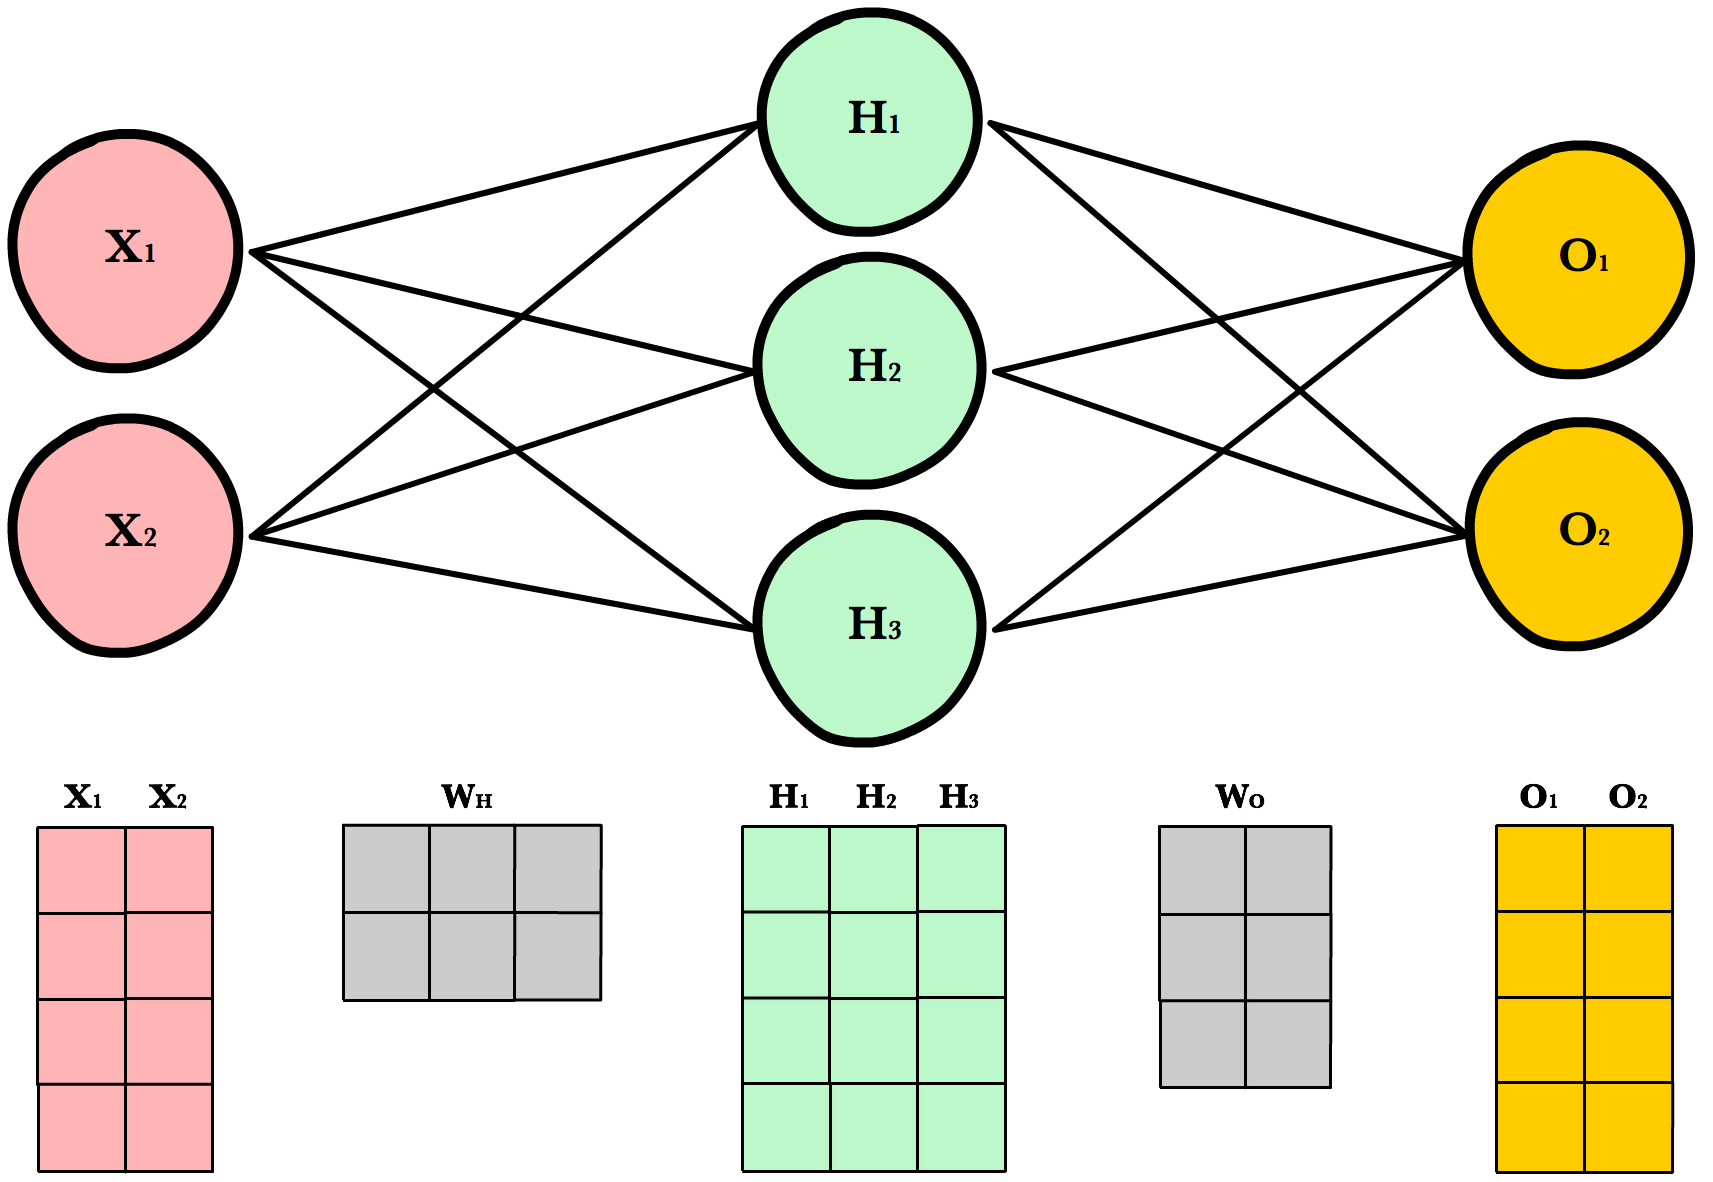
\includegraphics[width=0.85\textwidth]{img/neural_network_matrix_dense.png}
    \caption{Visualización de inferencia en redes neuronales densas}
    \label{fig:nn_matrix_dense}
\end{figure}

Así, si el dato (vectorial por la naturaleza de estas redes) tiene 24 elementos, será necesaria una capa de entrada de 24 neuronas (24 columnas $x_{1} .. x_{24}$ según notación de la Figura \ref{fig:nn_matrix_dense}), y si queremos inferir sobre 1000 de estos datos, esto se puede hacer en una sola ejecución, siendo el número de columnas también de 1000.

O dicho de otra manera, sea la capa $M_{m}$ una capa completamente conexa con $m$ neuronas, a la cual se le introduce un dato $x_{m}$, donde el peso de la neurona $M_{i}$ hacia $N_{j}$ se denota como $w_{M,i,j}$, y la función de transferencia es $\phi$, entonces se tiene que la salida de una capa será:

\begin{equation}
    x_{N,i} = \phi\left(\sum_{j}w_{N,i,j}x_{M,j}\right)\nonumber
    \label{eq:dense_nn_eq}
\end{equation}

A esta función se le puede añadir el \textit{bias} de forma explícita ($\sum\left([\dots] x_{M,j}\right) + bias_{N,i}$), o de forma implícita, siendo el \textit{bias} una conexión más, con un valor constante de 1, cuyo peso es el multiplicador que da el \textit{bias} resultante.

\section{Redes neuronales dispersas}
\label{sec:redes_reuronales_dispersas}
Las redes neuronales dispersas cuentan con una ventaja, y es el menor número de conexiones entre neuronas, o directamente el menor número de neuronas en la arquitectura. A pesar de esto, en realidad el fundamento matemático es el mismo, una simple multiplicación de matrices. Sin embargo, a pesar de tener el mismo funcionamiento base, se pueden explotar ciertas características, tanto de la estructura de las matrices dispersas como de su multiplicación, para obtener mejoras tanto en el tamaño del modelo como en su rendimiento, respectivamente.

\subsection{Fundamentos de matrices dispersas}
\label{ssec:fundamentos_matrices_dispersas}
Una matriz es dispersa cuando gran parte de su contenido son únicamente ceros. El cuan dispersa es una matriz se cuantifica mediante el ``grado de dispersión'' o \textit{sparsity}. Una matriz dispersa $10 \times 10$ con tres elementos diferentes de cero (denominados elementos \textit{nonzero} o directamente \textit{nonzeros}) será una matriz dispersa con una \textit{sparsity} del $97\%$ y una densidad del $3\% \:(=100\%-97\%)$.

\subsection{Almacenamiento de matrices dispersas}
\label{ssec:almacenamiento_matrices_dispersas}
Existen múltiples métodos para el almacenamiento de matrices dispersas en memoria, pero uno de los más sencillos de comprender, y que se usa en la \acrshort{poc} para la creación de las matrices dispersas, es el formato \acrshort{coo} o \textit{\acrlong{coo}}.

Este formato consiste en el almacenamiento de dato y coordenadas en tres vectores: \texttt{V}, \texttt{C} y \texttt{R} (\textit{Value}, \textit{Column}, \textit{Row}). Para cada entrada en el vector \texttt{V}, se crea una entrada en la misma posición para los vectores \texttt{C} y \texttt{R}, indicando la columna y fila en la que se ubica el valor \textit{nonzero}. Por diseño, el tamaño de cada uno de estos tres vectores tiene que ser igual al número de \textit{nonzeros}, denotado por \texttt{NZ}. Este formato es particularmente cómodo para la creación de matrices dispersas de forma ágil, pero existen formatos más avanzados, tanto en tamaño como en eficiencia, como el \acrshort{csr} o \textit{\acrlong{csr}}\footnote{Más información en \url{https://en.wikipedia.org/wiki/Sparse_matrix\#Compressed_sparse_row_(CSR,\_CRS\_or\_Yale\_format)}}.

A continuación se muestra un ejemplo de una matriz dispersa almacenada en formato \acrshort{coo}. A pesar de que esta matriz no es particularmente dispersa, se utiliza únicamente con fines explicativos:

\begin{center}
    $\begin{pmatrix}
        1 & 0 & 0 & 0\\
        0 & 2 & 0 & 0\\
        0 & 3 & 4 & 0\\
        0 & 0 & 0 & 5
    \end{pmatrix}$
    \vspace*{0.5cm}
\begin{lstlisting}[]
NZ = 5

V = [ 1 2 3 4 5 ]
C = [ 0 1 1 2 3 ]
R = [ 0 1 2 2 3 ]
\end{lstlisting}
\end{center}

\subsection{Propiedades del producto de matrices dispersas}
\label{ssec:propiedades_producto_matrices_dispersas}
Al multiplicar dos matrices densas no hay duda de que como resultado se obtendrá una matriz densa, salvo contadas excepciones, como multiplicar una matriz por su inversa. Sabiendo que el producto de matrices dispersas obtiene el mismo resultado que una multiplicación de matrices densas mediante un algoritmo diferente, se pueden clasificar los productos de matrices en función de su \textit{sparsity} de forma genérica.

Esta clasificación, de nuevo, puede variar en función de las propiedades de la matriz, pero es la base sobre la cual se construyen las funciones de \acrshort{blas} (\textit{\acrlong{blas}}) \cite{netlib_blas} y las implementaciones Sparse BLAS \cite{sparse_blas_10.1145/567806.567810}. De esta forma, se pueden implementar los siguientes tipos de producto de matrices:

\begin{itemize}
    \item Densa $\times$ Densa $=$ Densa ($D\times D$)
    \item Dispersa $\times$ Densa $=$ Densa ($d\times D$)
    \item Dispersa $\times$ Dispersa $=$ Dispersa / Densa\footnote{En función de la forma en que los valores \textit{nonzero} estén dispuestos en ambas matrices, el resultado puede ser una matriz dispersa o densa.} ($d\times d$)
\end{itemize}

Estos tres tipos principales de productos, en típico \textit{BLAS-fashion} se pueden realizar para tipos de datos según su precisión, \texttt{S}, \texttt{D}, \texttt{C} y \texttt{Z} (\textit{Single}, \textit{Double}, \textit{Single Complex}, \textit{Double Complex}).
Así, se pueden obtener las siguientes funciones estándar, a pesar de que en la parte \textit{sparse} de \acrshort{blas} hay menor consenso debido a la existencia de múltiples librerías que difieren del estándar por ser previas a la creación del mismo. Por ejemplo, los tipos especificados en la función se van perdiendo conforme se avanza hacia implementaciones genéricas en C++.

\begin{itemize}
    \item \texttt{[sdcz]gemm()} para $D\times D$
    \item \texttt{[sdcz]usmm()} o \texttt{spmm()} para $d\times D$
    \item \texttt{sp[sdcz]gemm()} o \texttt{spmsp()} para $d\times d$
\end{itemize}

Sabiendo las características de una red neuronal dispersa, y tal como se comenta más adelante en esta memoria, en la \acrshort{poc} se emplea el producto $d\times D$, debido a la naturaleza dispersa de los pesos, y densa de los datos de entrada. De todas formas, en función de la naturaleza de los datos de entrada, podrían emplearse también vectores de entrada dispersos, aunque lo más probable es que para eso quizás una red neuronal \textit{feed-forward} unidimensional no sea lo más apropiado, y ya se deban sugerir otras arquitecturas de red como las convolucionales, debido a que un vector disperso no suele tener mucho sentido, pero una matriz dispersa sí.
x
\subsection{Visualización de una red neuronal dispersa}
\label{ssec:visualizacion_nn_dispersa}
Tal como se mostró en la Sección \ref{sec:redes_reuronales_densas}, es sencillo visualizar el proceso de inferencia como una simple multiplicación de matrices, por lo que una multiplicación con una matriz de pesos dispersa debería ser sencilla de visualizar de forma similar.

Y este razonamiento es correcto, es muy sencilla de visualizar de no ser por un pequeño detalle. Y es que la función de multiplicación de matrices $d\times D$, \texttt{[sdcz]usmm()}, tiene una firma poco genérica, haciendo que, si bien esta función parezca adecuada para esta carga de trabajo, tenga un sutil detalle que requiere un poco de detenimiento. A continuación se muestra para el lenguaje C y para simple precisión la firma y parámetros de la función \texttt{BLAS\_susmm}:

\begin{lstlisting}[language=C]
int BLAS_susmm( enum blas_order_type    order,
                enum blas_trans_type    transA,
                int                     nrhs,
                float                   alpha,
                blas_sparse_matrix      A,
                const float *           b,
                int                     ldb,
                float *                 c,
                int                     ldc 
)

/**
 * order    Layout of the dense array.
 * transA   Transposition operator for matrix A.
 * nrhs     Number of right hand side columns.
 * A        A valid matrix handle.
 * alpha    Value for alpha.
 * b        Dense vector b.
 * ldb      Leading dimension of b.
 * c        Dense vector c.
 * ldc      Leading dimension of c.
 */
\end{lstlisting}

El inconveniente de esta función, que calcula $C = \alpha AB + C$, es que la matriz $A$ debe ser dispersa, algo que, fijándose de nuevo en la Figura \ref{fig:nn_matrix_dense}, no se cumple. Es decir, la matriz dispersa es la de pesos $w$, por lo que parece necesaria una función que trate a $B$ como una matriz dispersa. Dicha función no existe.

\begin{figure}[h!]
    \centering
    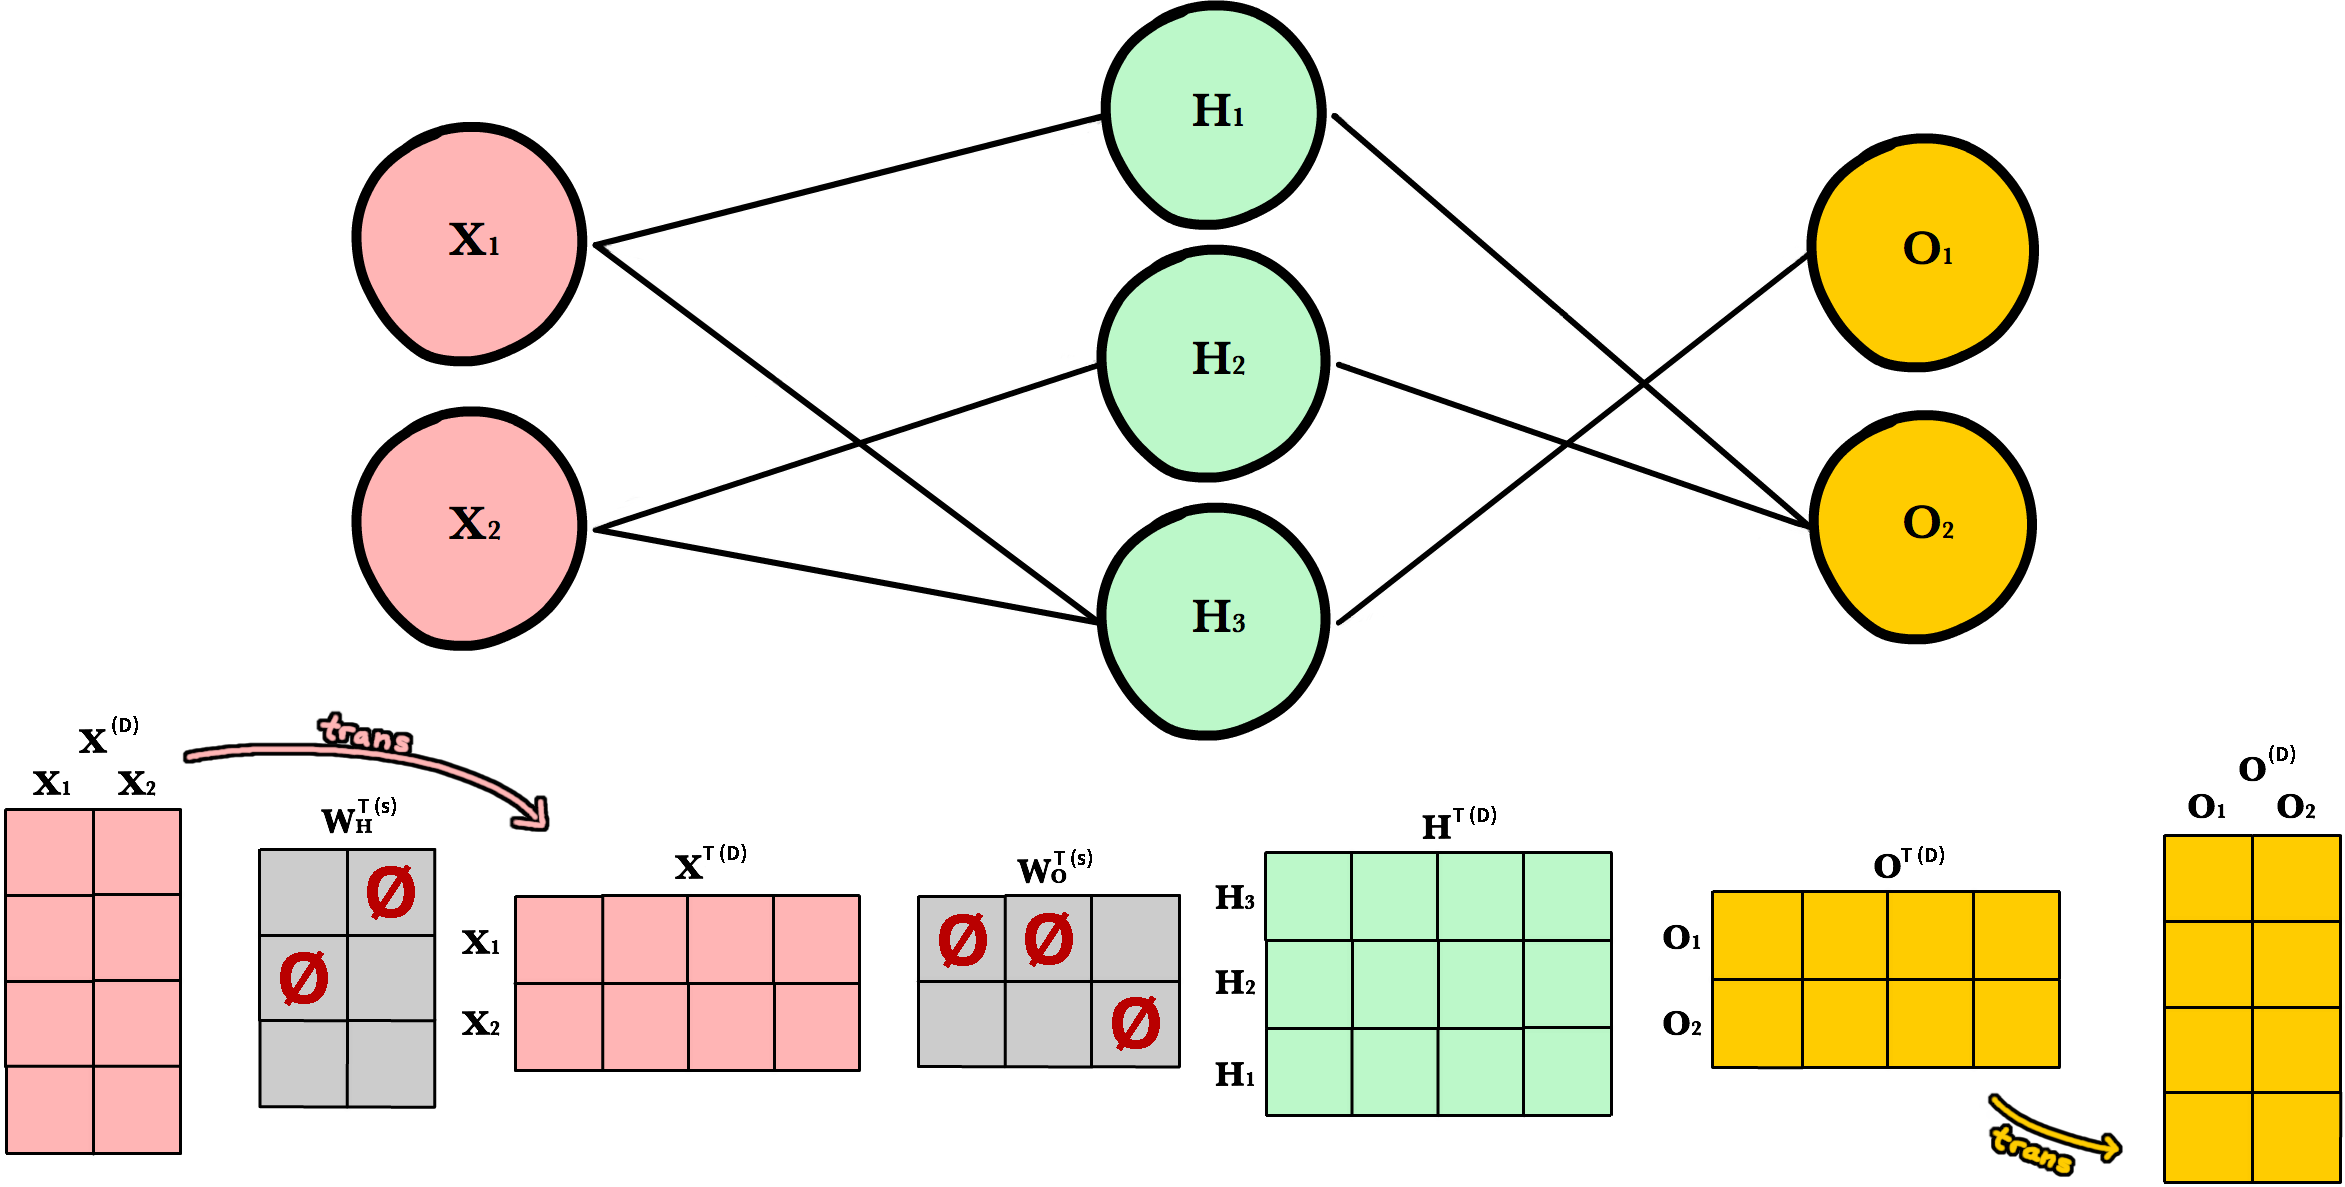
\includegraphics[width=\textwidth]{img/neural_network_matrix_sparse/neural_network_matrix_sparse.png}
    \caption{Visualización de inferencia en redes neuronales dispersas}
    \label{fig:nn_matrix_sparse}
\end{figure}

Sin embargo, empleando las propiedades de las matrices, es posible modificar el orden de las mismas, y así poder encajar cada matriz en la firma. Para esto se emplea una propiedad básica de las matrices, $C^{T} = (AB)^{T} = A^{T}B^{T}$. De esta forma, al transponer la matriz de pesos mediante el parámetro \texttt{transA}, y multiplicando esto por la salida de la capa anterior, se obtiene la salida $C^{T}$. Esto supone un pequeño overhead, al tener que transponer la entrada a la capa de entrada, así como la salida de la capa de salida. Sin embargo, dicho overhead puede mitigarse en gran medida, en función de la arquitectura de la red, así como de la fuente de datos, que es más que probable que mediante pequeñas modificaciones como filtrado o manejo de ficheros pueda exportar los datos transpuestos de base.

Esta estrategia se puede apreciar en la Figura \ref{fig:nn_matrix_sparse}, donde a diferencia de la Figura \ref{fig:nn_matrix_dense} se han transpuesto los pesos y las entradas, y han sido etiquetados correspondientemente mediante superíndices.

\section{Multiplicación de matrices \textit{point-to-point}}
\label{sec:multiplicacion_point_to_point}
A pesar de todo lo comentado previamente, el empleo de las funciones que ofrecen Sparse BLAS, Intel MKL\footnote{\url{https://www.intel.com/content/www/us/en/develop/documentation/get-started-with-mkl-for-dpcpp/top.htmlde ver}} y alternativas, no es la única opción para realizar la multiplicación de matrices dispersas. Una buena aproximación es el empleo de una arquitectura \textit{point-to-point}, \textit{fully unrolled} o \textit{data-specific}. Esta arquitectura consiste en \textit{hardcodear} cada una de las operaciones que intervienen en la multiplicación de matrices dispersas con una línea de \texttt{\acrshort{fma}} (\textit{\acrlong{fma}}) por cada valor no cero (\textit{point}) de la matriz.

Para generar dicho código se necesita tener primero una base teórica. Consideremosm el siguiente ejemplo: sean dos matrices $d \times D$, de dimensiones $m \times n$ y $n \times k$, respectivamente, teniendo la matriz dispersa una densidad del 50\%, y siendo $\#nz$ el número de valores \textit{nonzero} en la misma:
\begin{gather}
    \begin{pmatrix}
        0 & d_{12}\\
        d_{21} & 0\\
        0 & d_{32}
    \end{pmatrix}	
    \begin{pmatrix}
        D_{11} & \dots\\
        D_{21} & \dots
    \end{pmatrix}
    =
    \begin{pmatrix}
        C_{11} & \dots\\
        C_{21} & \dots\\
        C_{31} & \dots
    \end{pmatrix} \nonumber % https://latex.org/forum/viewtopic.php?t=20368
\end{gather}

Comenzando con la matriz resultado $C$ en una región de memoria a cero, la secuencia de operaciones a realizar sería la siguiente para este ejemplo:
\begin{center}
    $C_{11} \pluseq d_{12} \cdot D_{21}$\\
    $C_{21} \pluseq d_{21} \cdot D_{11}$\\
    $C_{31} \pluseq d_{32} \cdot D_{21}$\\
\end{center}

Esta secuencia \textit{hardcodeada} se repetirá $k$ veces (el número de columnas de $D$ y $C$). Teniendo en cuenta que una operación \texttt{\acrshort{fma}} realiza dos FLOPs, se puede concluir que el número de FLOPs necesarios para el cálculo de la matriz resultado $C$ será $2 \cdot \#nz \cdot k$.

\subsection{Teoría y ventajas de la localidad}
\label{ssec:teoria_ventajas_localidad}
Teniendo en cuenta que, para la matriz de pesos dispersa, sus valores \textit{nonzero} pueden almacenarse en memoria de forma secuencial, y dada la propiedad asociativa de la suma, se puede conseguir un algoritmo de multiplicación de matrices que únicamente realice accesos por filas. Al fin y al cabo todo se reduce a cómo se representan las matrices en memoria.

Por tanto, para una multiplicación de matrices similar a la tratada en esta sección ($w^{d} \times x^{D} = out^{D}$, de dimensiones $m \times n$, $n \times k$ y $m \times k$, respectivamente), se puede representar la dimensión común de medida $n$ en el eje horizontal. La siguiente multiplicación de matrices no está en una disposición compatible, pero tal como se puede apreciar en la siguiente subsección, tenerlas en este \textit{layout} en memoria es muy beneficioso para la localidad de los datos: 
\begin{gather}
    \begin{pmatrix}
        w_{00} & w_{01}\\
        0 & w_{11}\\
        0 & 0\\
        w_{30} & w_{31}
    \end{pmatrix}	
    \begin{pmatrix}
        x_{00} & x_{01}\\
        x_{10} & x_{11}\\
        \vdots & \vdots
    \end{pmatrix}
    =
    \begin{pmatrix}
        out_{00} & out_{01} & out_{02} & out_{03}\\
        out_{10} & out_{11} & out_{12} & out_{13}\\
        \vdots & \vdots & \vdots & \vdots
    \end{pmatrix} \nonumber
\end{gather}

\subsection{Obtención de la secuencia de operaciones}
\label{ssec:obtencion_secuencia_operaciones}
El procedimiento a seguir será multiplicar cada una de las filas de la matriz $w^{d}$ por cada fila de la matriz $x^{D}$, ambas mostradas en la subsección anterior. A cada iteración de la matriz $w^{d}$ se desplazará una posición a la derecha en la matriz $out^{D}$. Sin embargo, primero es conveniente almacenar los valores dispersos de la matriz $w^{d}$. Para esto, se puede construir una \acrshort{lut} (\textit{\acrlong{lut}}). En esta tabla se almacenan cada uno de los valores \textit{nonzero} de la matriz $w^{d}$ recorrida en orden secuencial estilo C. Para este ejemplo, el contenido de la \acrshort{lut} se muestra en la Tabla \ref{tab:lut_example}. En la columna izquierda puede verse la coordenada original del valor ubicado en la posición a su derecha.

\begin{table}[h!]
    \centering
    \begin{tabular}{|c|c|}
    \hline
    \textbf{(x$^{\sharp}$,y$^{\flat}$)} & \textbf{pos$^{\natural}$} \\\hline
    (0,0) & 0 \\\hline
    (0,1) & 1 \\\hline
    (1,1) & 2 \\\hline
    (3,0) & 3 \\\hline
    (3,1) & 4 \\\hline
    \end{tabular}
    \caption{Contenido de la LUT para la matriz $w^{d}$. \textbf{x}, \textbf{y} y \textbf{pos} se etiquetan con $\sharp$, {\large$\flat$} y $\natural$}
    \label{tab:lut_example}
\end{table}

A su vez, en la Tabla \ref{tab:w_matrix_memory_layout} se puede ver la disposición en memoria de cada valor \textit{nonzero} de la matriz dispersa de pesos que, debido a la omisión de los ceros en $w^{d}$ se almacenan forma contigua en memoria.

\begin{table}[h!]
    \centering
    \begin{tabular}{|c|c|c|c|c|c|}
        \hline
        \textbf{pos} & 0 & 1 & 2 & 3 & 4 \\\hline
        \textbf{val} & $w_{00}$ & $w_{01}$ & $w_{11}$ & $w_{30}$ & $w_{31}$ \\\hline
    \end{tabular}
    \caption{Disposición en memoria de los valores \textit{nonzero} de la matriz $w^{d}$}
    \label{tab:w_matrix_memory_layout}
\end{table}

Como el almacenamiento de matrices e C es por filas, se pueden tomar punteros al inicio de cada una de las filas en las matrices $x^{D}$ y $out^{D}$ y repetir esta secuencia $k$ veces. Es importante recordar que, aunque los accesos a la matriz $w^{d}$ sean aleatorios, sus valores son accedidos secuencialmente. De esta forma, se recorre cada una de las entradas de la \acrshort{lut}, tomando cada índice etiquetado con $\sharp$, $\flat$ y $\natural$ en la Tabla \ref{tab:lut_example} tal como se indica a continuación:

\begin{center}
    $out = base\_out + m*num\_iteracion$\\
    $D = base\_D + n*num\_iteracion$\\
    \ \\
    \ \ \ \ \ \  $\sharp$ \ \ \ \ \ \ \ \ \ \ \ \ \  $\natural$ \ \ \ \ \ \ \ \  {\large$\flat$} \ \\
    $out[0] \pluseq w[0] \cdot D[0]$\\
    $out[0] \pluseq w[1] \cdot D[1]$\\
    $out[1] \pluseq w[2] \cdot D[1]$\\
    $out[3] \pluseq w[3] \cdot D[0]$\\
    $out[3] \pluseq w[4] \cdot D[1]$\\
\end{center}

\section{TensorFlow}
\label{sec:tensorflow}
Por último, en este capítulo es conveniente hablar de \acrlong{tf} (frecuentemente abreviado como \acrshort{tf}). Siendo una de las librerías de código abierto más ampliamente empleadas en la industria, esta es la librería empleada en el Capítulo \ref{chap:desarrollo_poc} para la creación del modelo, permitiendo así omitir todos los detalles de implementación en el proceso de entrenamiento.

Creado por Google para el desarrollo de modelos de aprendizaje automático, \acrlong{tf} expone \acrshort{api}s para Python, C++ y muchos otros lenguajes. Asimismo \acrlong{tf} permite la ejecución de código en CPU, GPU y TPU y, además, debido a su naturaleza \textit{open source}, está abierta a modificaciones que implementen \textit{\gls{backend}s} de hardware XPU específicos.

Al ser una librería tan grande, conocida y predominante en la industria, se puede encontrar una gran cantidad de redes neuronales preentrenadas, fácilmente importables a \acrlong{tf}, en formatos tales como \texttt{.onnx}, \texttt{.pb} o \texttt{.npz}, en proyectos como el \textit{ONNX Model Zoo}\footnote{\url{https://github.com/onnx/models}}.

En este trabajo se emplea la \acrshort{api} de Python para el modelado, creación, podado y correspondientes entrenamientos del modelo. Todos los códigos exportados en formatos compatibles con \acrlong{tf}, así como códigos C para todas las arquitecturas previamente descritas, se pueden encontrar bajo \texttt{res/} en la raíz del proyecto\footnote{\url{https://github.com/forcegk/HPC_TFM}}.
% \include{contido/analisis_diseño}
% \include{contido/implementacion}
% \chapter{Medida del rendimiento y perfilado}
\label{chap:medida_rendimiento_perfilado}

\lettrine{E}{n} este capítulo, tras plantear la problemática y se documentar cómo se construye la prueba de concepto en los capítulos anteriores, se muestran los resultados de las medidas de rendimiento tanto para los códigos densos como dispersos. Estos resultados se comparan con los que se pueden ver en la literatura ya existente, para comprobar si la red implementada se adhiere a los patrones indicados por ejemplo en la Sección \ref{sec:investigacion_optimizaciones_propuestas}.

\section{Metodología}
\label{sec:metodologia}
La medida del rendimiento de las pruebas de concepto no es tarea trivial. Al ser una simple Prueba de Concepto la función \texttt{map\_and\_bias} no está debidamente optimizada con OpenMP. Realizar esta optimización no es difícil, pero quizás sería innecesario cuando lo que se pretende es medir las posibilidades de una aproximación, y no optimizar y trabajar a fondo en ella.

Por esta razón se ha decidido simplemente implementar de forma sencilla la generación de código con las librerías OpenBLAS y librsb, sin añadir OpenMP u optimizaciones mayores en funciones auxiliares. El \textit{overhead} que añade el tratamiento auxiliar de datos es lo suficientemente bajo como para no necesitar paralelización en un entorno de pruebas.

\subsection{Común}
\label{ssec:comun_metodologia}
Para la medida del rendimiento y perfilado se generan dos redes neuronales de un tamaño absurdamente grande, una densa con capas completamente conexas con un anchos tal que \{capa de entrada, $n\:\times\:$capas ocultas, capa de salida\} = \{24, 500, 800, 1000, 1200, 600, 400, 200, 100, 50, 1\}, y otra dispersa con una \textit{sparsity} del 95\% generada a partir del modelo denso. Evidentemente, para el problema que se pretende resolver, estas redes están completamente sobredimensionadas y son cuanto menos inútiles, puesto que debido a su enorme tamaño lo único que aprenden durante el proceso de entrenamiento es a marcar como positivos todos los \textit{inputs}.

Esto, que para un ingeniero en inteligencia artificial sería un enorme fracaso, en este ámbito es algo completamente indiferente, ya que a pesar de la inutilidad de la red creada, esta sigue realizando las cargas de trabajo típicas de una red neuronal adecuada, esto es, multiplica matrices, suma los \textit{bias} y aplica funciones de transferencia.

En ambas ejecuciones se emplean los mismos datos de entrada, que consisten en el fichero \texttt{input.txt} generado con la función tratada en el Punto 3 de la Sección \ref{ssec:extraccion_valores}, replicado 100 veces, para obtener $1000 \times 100 = 100000$ datos de entrada.

\subsection{Medida del rendimiento}
\label{ssec:medida_rendimiento_metodologia}
Para la medida del rendimiento se emplea el programa \texttt{hyperfine}\footnote{\url{https://github.com/sharkdp/hyperfine}} y compilaciones de \textit{release} (opción \texttt{-s} o \textit{strip}). Mediante esta herramienta se realizan 15 ejecuciones de las cuales se calcula la media y desviación típica automáticamente, con 3 ejecuciones previas de calentamiento. Siendo un ejemplo de binario generado \texttt{dense.out}, la ejecución del \textit{benchmark} sería tal que:\medskip
\begin{lstlisting}[language=bash]
hyperfine --warmup 3 --runs 15 './dense.out input.txt'
\end{lstlisting}

Tanto las ejecuciones de medición de tiempos como los perfilados se realizan en un equipo Xiaomi Mi Notebook 15 con las características visibles en la Tabla \ref{tb:especificaciones_xiaomi}.
\begin{table}
\centering
\begin{tabular}{|c|c|}
    \hline
    CPU & 11th Gen Intel(R) Core(TM) i7-11370H @ 3.30GHz\\\hline
    RAM & 16 GB @ 3200MHz (Dual Channel)\\\hline
    Sistema & Ubuntu 20.04 - Linux TODO COMPLETAR\\\hline
    CC & gcc 11 TODO CHECKEAR VERSIÓN\\\hline
    OpenBLAS & libopenblas-dev focal, v0.3.8\\\hline
    librsb & librsb-dev focal, v1.2.0.8\\\hline
    oneapi & Intel oneAPI 2022\\\hline
\end{tabular}
\caption{\label{tb:especificaciones_xiaomi}Especificaciones técnicas del equipo de pruebas}
\end{table}


\subsection{Análisis y perfilado}
\label{ssec:analisis_perfilado_metodologia}
Para el análisis y perfilado se emplea el programa Intel Advisor, el cual permite realizar modelos \textit{roofline} de partes individualizadas de programas, incluyendo las funciones de su librería \acrshort{mkl} (\textit{\acrlong{mkl}}). Esto es especialmente útil para perfilar la implementación densa, que emplea funciones de \texttt{cblas} ampliamente utilizadas.

Sin embargo, esta universalidad se pierde con la versión dispersa (\textit{sparse}), ya que se emplean funciones \textit{built-in} de OpenBLAS, así como funciones propias de librsb, lo que hace que cambiar a la \acrshort{mkl} requiera una reprogramación de ciertas líneas del código para poder perfilar las funciones de librería con Intel Advisor. Esto, que inicialmente puede parecer un problema, no lo es tanto si se razona con respecto al \textit{roofline} de la versión densa.

\subsection{Compilación}
\label{ssec:compilacion_metodologia}
Para compilar las versiones densa y dispersa se requiere intercambiar OpenBLAS por la Intel \acrshort{mkl}, así como desactivar el \textit{stripping} del binario para activar los símbolos de depuración (susituir parámetro \texttt{-s} por \texttt{-g}). Esto implica modificar las líneas de compilación genéricas que se pueden encontrar en el fichero \texttt{.ipynb}, tal como se muestra a continuación.

\subsubsection{Código denso}
Para la obtención del \textit{roofline model} de la carga de trabajo, es necesario o bien calcularlo manualmente, o bien emplear alguna herramienta adecuada para ello. Como ya se comenta previamente, se emplea Intel Advisor para el perfilado del código, por lo que es necesario compilar el código denso con una configuración que sustituya OpenBLAS por \acrshort{mkl}. Para esto se puede compilar de las siguientes formas:\medskip
\begin{lstlisting}[language=bash]
# Para una compilación convencional sin depuración con OpenBLAS, sería necesario únicamente ejecutar
gcc -march=native -O3 -s *.c -o dense.out -lm -lcblas       # En Arch Linux
gcc -march=native -O3 -s *.c -o dense.out -lm -lopenblas    # En Ubuntu

# Sin embargo, con propósitos de perfilado con Intel Advisor, en un entorno bash donde se haya realizado `source /opt/intel/oneapi/setvar.sh` se ha de compilar con:
gcc -march=native -O3 -g3 -DMKL_ILP64 -m64 -I"${MKLROOT}/include" *.c -o dense.out -L${MKLROOT}/lib/intel64 -Wl,--no-as-needed -lmkl_intel_ilp64 -lmkl_gnu_thread -lmkl_core -lgomp -lpthread -lm -ldl
\end{lstlisting}

\subsubsection{Código \textit{sparse}}
En este caso, debido al uso de \texttt{librsb} como librería de Sparse BLAS, la herramienta de perfilado y análisis de código Intel Advisor, a pesar de recompilar la librería con \textit{flags} de \textit{debug}, no es capaz de analizar el código de librería. Una adaptación a la librería Intel MKL, a pesar de no ser imposible, no es conveniente. Por esto mismo más adelante en este capítulo se estima el rendimiento y posibilidades de mejora del código disperso, en función a los resultados con respecto al denso. Para compilar el código para \textit{release}, las líneas de compilación son las siguientes:\medskip
\begin{lstlisting}[language=bash]
# Para una compilación convencional sin depuración con OpenBLAS, sería necesario únicamente ejecutar
gcc -march=native -O3 -s *.c -o sparse.out -lm -lrsb -lcblas # En Arch Linux
gcc -march=native -O3 -s *.c -o sparse.out -lm -lrsb -lopenblas  # En Ubuntu
\end{lstlisting}

\section{Medida de rendimiento, perfilado y \textit{roofline model}}
\label{sec:medida_perfilado_roofline}
En esta sección se muestran los resultados obtenidos según la metodología descrita en la sección anterior, así como se razonan los posibles resultados que no se han podido obtener debido a limitaciones en el análisis.

\subsection{Código denso}
Los resultados obtenidos para la red neuronal densa son los siguientes:

\begin{center}
Tiempo $(\overline{t} \pm \sigma)$ = 10,300 s $\pm$ 0,152 s

Rangos (min \ldots\ max) = 10,022 s \ldots\ 10,568 s
\end{center}

Estos resultados se obtienen además realizando un excelente uso de la memoria caché, tal como se muestra en el modelo \textit{roofline} en la Figura \ref{fig:roofline_dense}.

\begin{figure}[h!]
    \centering
    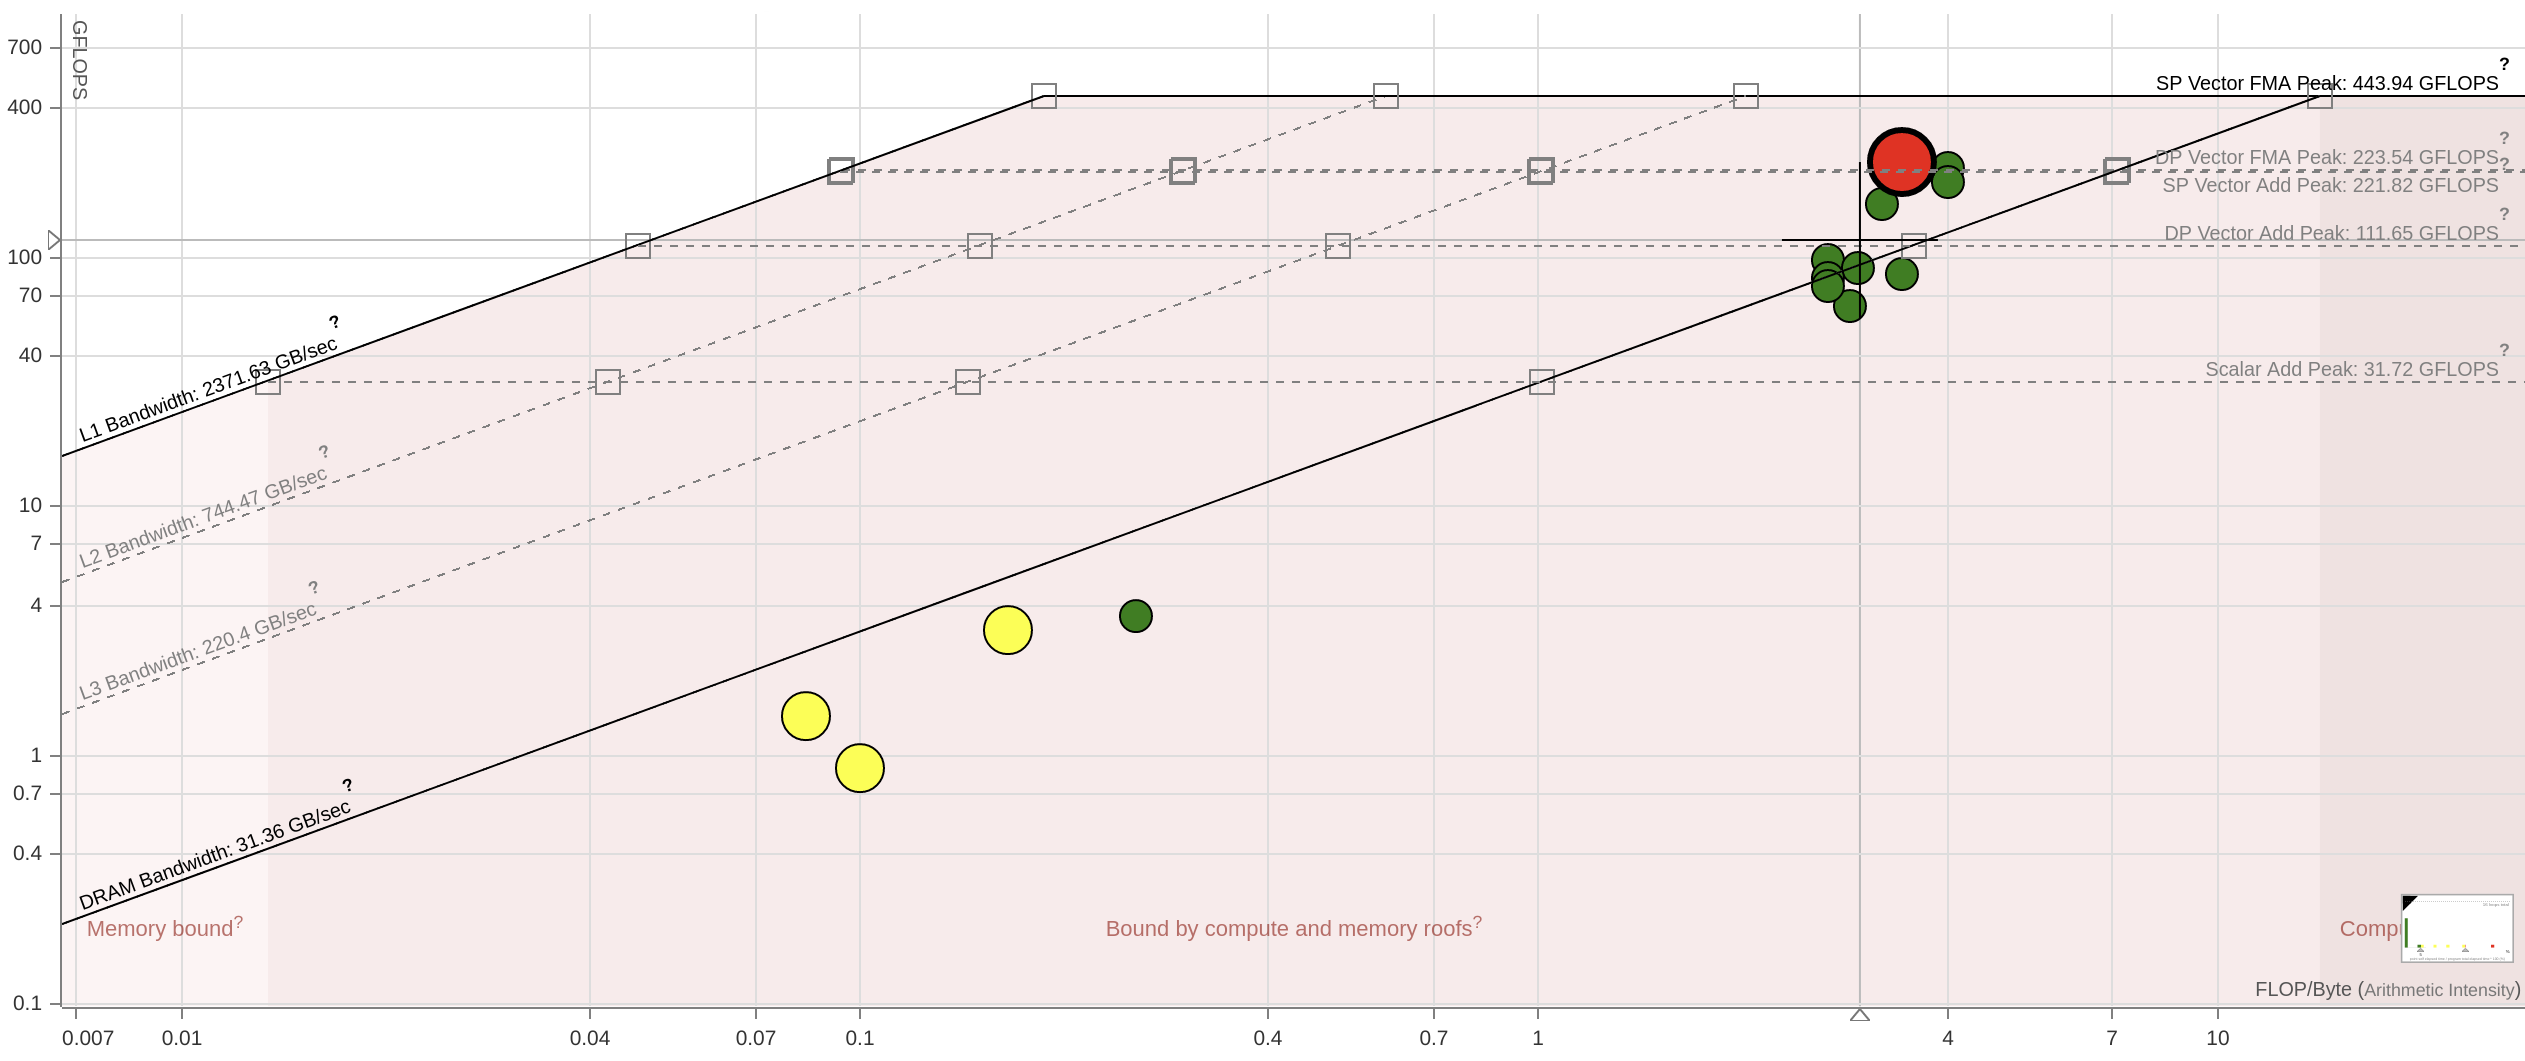
\includegraphics[width=\textwidth]{img/roofline_dense.png}
    \caption{\textit{Roofline model} del código denso}
    \label{fig:roofline_dense}
\end{figure}

Como se puede apreciar en el modelo, el \textit{workload} de interés, que es el que se puede encontrar en la parte superior derecha (coloreado en rojo y verde), corresponde a las funciones \texttt{cblas\_sgemm}. Estas funciones están fuertemente optimizadas y emplean instrucciones AVX512, como se puede observar en los detalles de la carga (Figura \ref{fig:roofline_dense_details}).

Fijándose con atención se pueden ver funciones con un considerablemente menor desempeño en la parte inferior izquierda. Estos puntos corresponden a \texttt{map\_and\_bias} y sucesivas llamadas a otras funciones como \texttt{expf}. Tal como se comenta previamente, una paralelización es sencilla de funciones auxiliares es sencilla. Sin embargo y tal como se puede ver en el modelo, se pueden distinguir perfectamente los componentes de dichas funciones, y siendo el tiempo de ejecución constante para dos redes con las mismas dimensiones, es sencillo discernir qué mejorías vienen causadas por un producto de matrices más eficiente.    

\begin{figure}[h!]
    \centering
    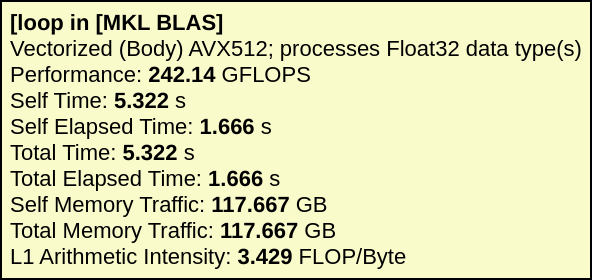
\includegraphics[width=0.5\textwidth]{img/roofline_dense_details.png}
    \caption{Detalles de \texttt{cblas\_sgemm} en el modelo del código denso}
    \label{fig:roofline_dense_details}
\end{figure}

\subsection{Código \textit{sparse}}
Por otro lado, los resultados obtenidos para la red neuronal dispersa son los siguientes:

\begin{center}
Tiempo $(\overline{t} \pm \sigma)$ = 13,862 s $\pm$ 0,710 s

Rangos (min \ldots\ max) = 12,635 s \ldots\ 15,285 s
\end{center}

En este caso, debido al empleo de la librería librsb, el modelo \textit{roofline} no contiene información de utilidad (Figura \ref{fig:roofline_sparse_details}). Esto, que a todas luces es un problema, deja de serlo si se realiza un sencillo razonamiento.

\begin{figure}[h!]
    \centering
    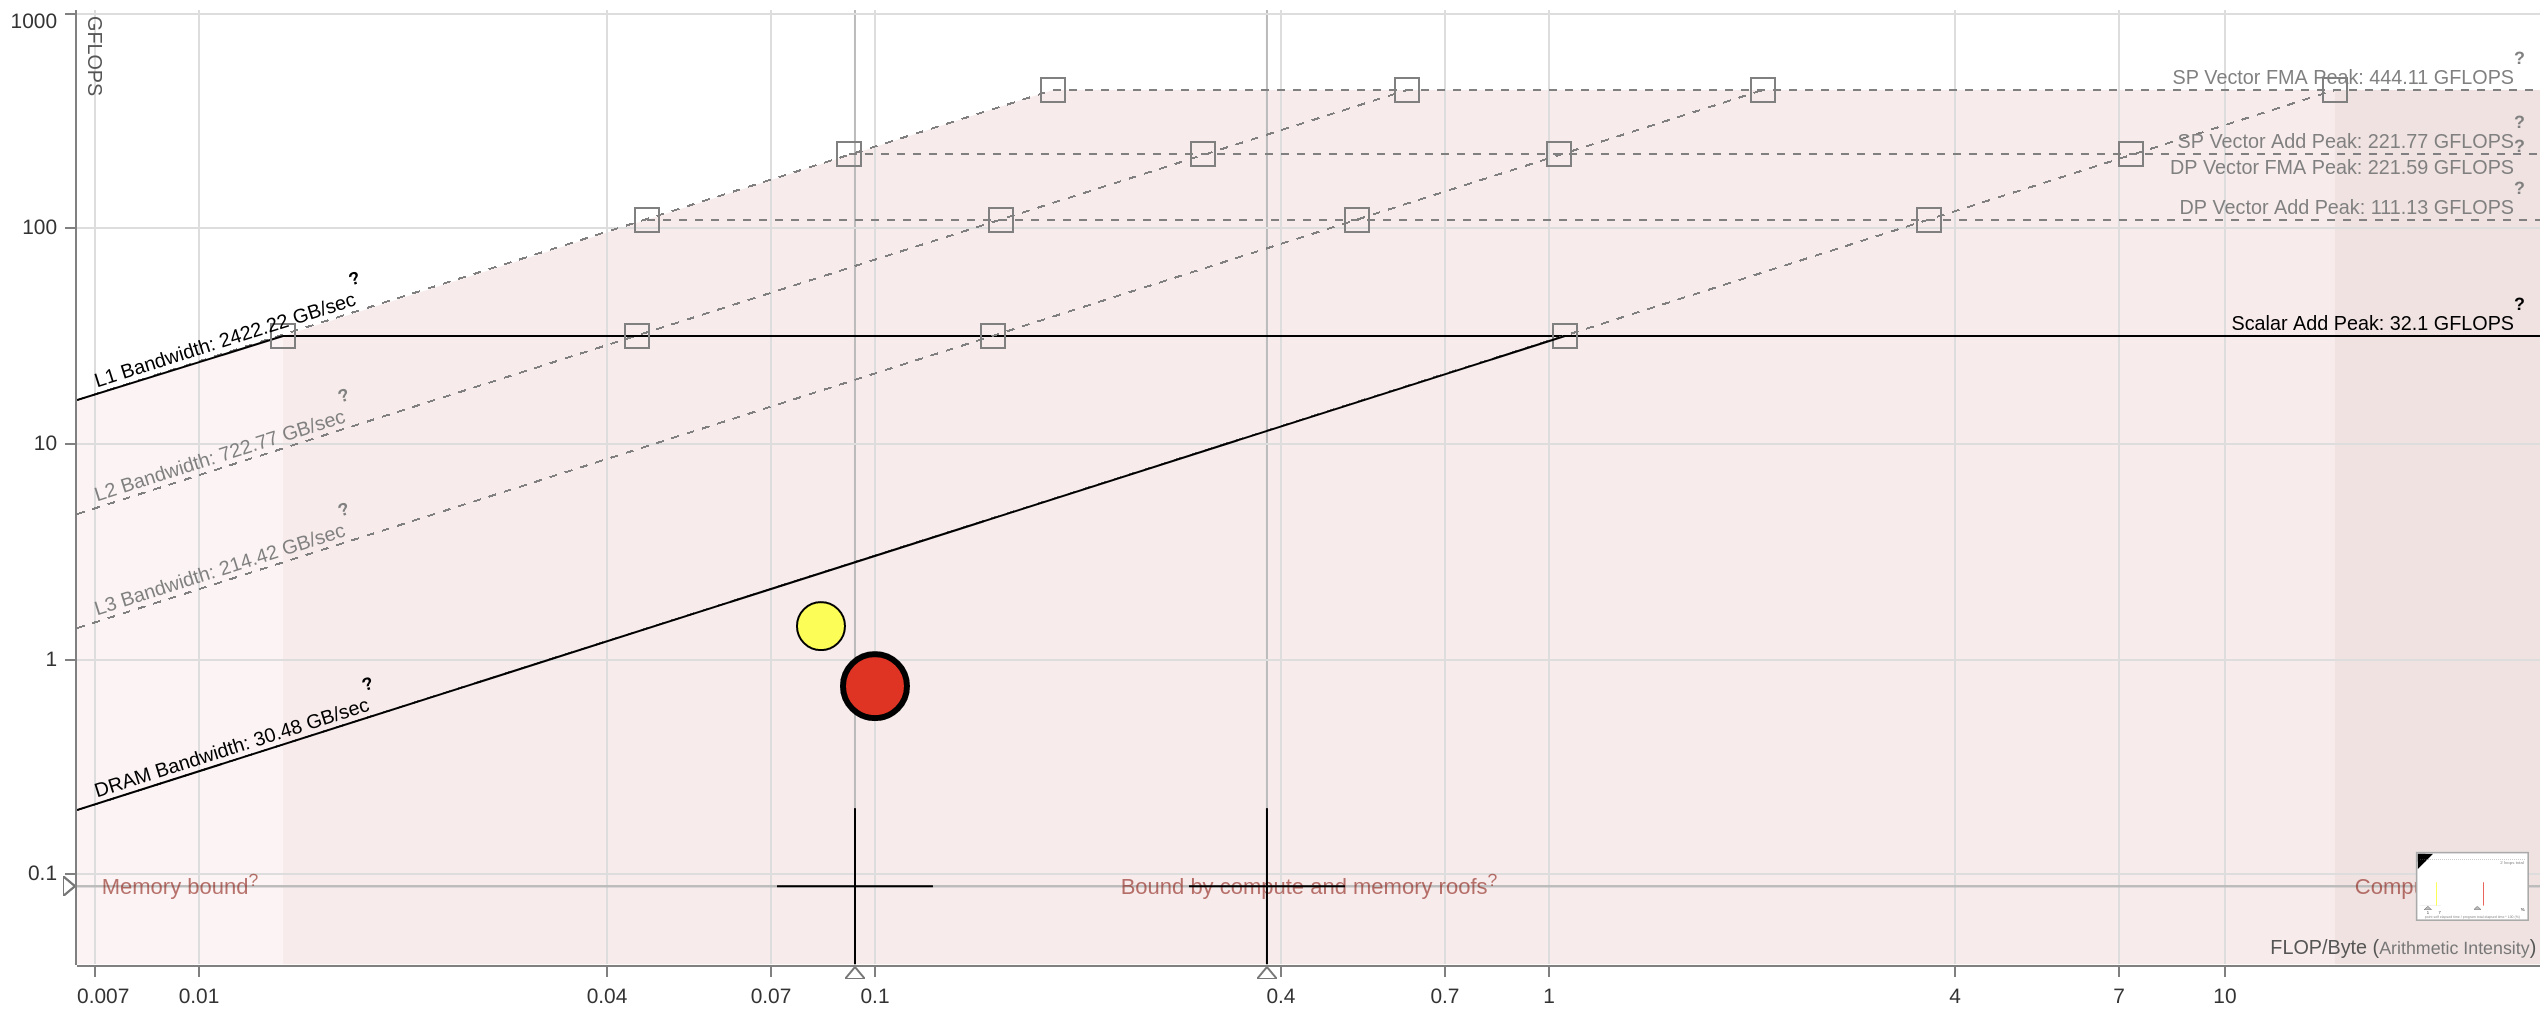
\includegraphics[width=\textwidth]{img/roofline_sparse.png}
    \caption{\textit{Roofline model} del código disperso}
    \label{fig:roofline_sparse_details}
\end{figure}

Teniendo en cuenta que los tiempos de ejecución de una red dispersa al 95\% son \textasciitilde25\% superiores a los de la red completamente conexa, aún teniendo que procesar un 95\% menos de datos, se puede realizar una estimación del número teórico de FLOP necesarios para las operaciones de multiplicación.

\subsubsection{Aproximación teórica}
Tal como se explica en la Sección \ref{sec:multiplicacion_point_to_point}, teniendo en cuenta que una operación FMA realiza dos FLOP, se puede concluir que el número de FLOP para la multiplicación de dos matrices $d\times D$ será $2 \cdot \#nz \cdot k$.

\subsubsection{Estimación del rendimiento}
Teniendo en cuenta que las matrices dispersas de pesos en el código disperso tienen una densidad del 5\% (o lo que es lo mismo, una \textit{sparsity} del 95\%), desde un punto de vista teórico se puede concluír que se deberían realizar un 95\% menos de operaciones en punto flotante.

Sin embargo esta reducción en el número de operaciones necesarias, debido a múltiples factores como el principio de localidad, estructura interna a la hora de almacenar la matriz, estructuras de control, así como optimizaciones internas de la propia librería, no se corresponde con una disminución del tiempo de ejecución, sino más bien todo lo contrario. Esta reducción en el número de FLOPS no lo es sin embargo en intensidad aritmética, puesto que también se cuenta con menor número de bytes de datos, resultando en un hipotético descenso en el eje $y$ en el modelo.

Por esta razón, el modelo \textit{roofline} resultante, que el programa Intel Advisor es incapaz de generar, se vería similar a lo que se puede observar en la Figura \ref{fig:roofline_sparse_estimado}.

\begin{figure}[h!]
    \centering
    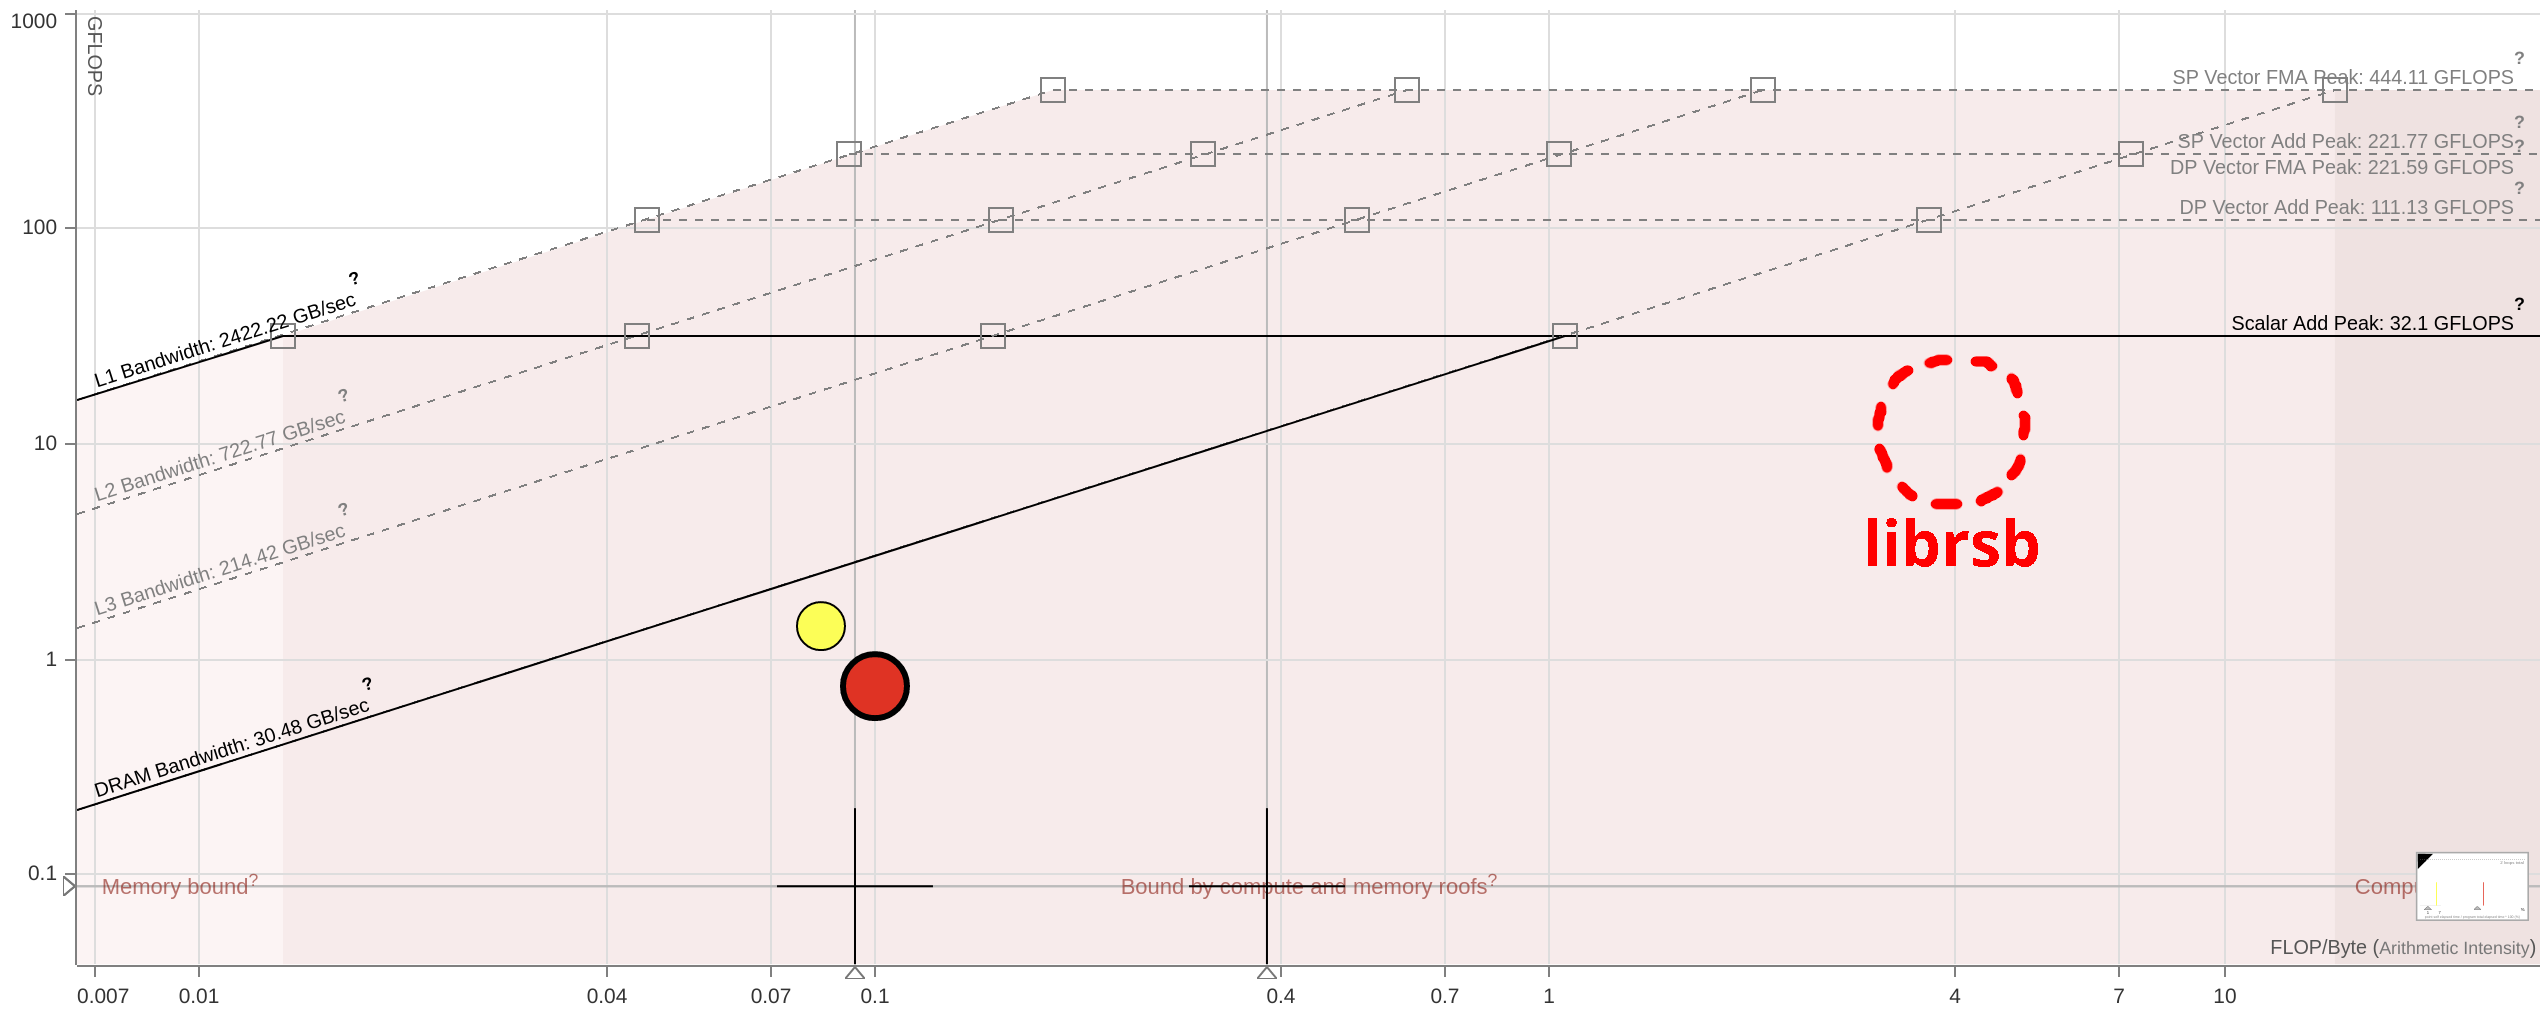
\includegraphics[width=\textwidth]{img/roofline_sparse_estimado.png}
    \caption{Estimación del \textit{roofline model} del código disperso}
    \label{fig:roofline_sparse_estimado}
\end{figure}

Estos decepcionantes resultados, sin embargo, no son tan desalentadores, ya que implica que existe un amplio margen de mejora mediante análisis estático de código y generación de instrucciones FMA y de control \textit{ad-hoc}, que incluso pueden ser vectorizadas mediante el empleo de la herramienta MARTA\footnote{\url{https://github.com/UDC-GAC/MARTA}}.
% \include{contido/aplicacion_web}
% \include{contido/planificacion_costes}
\chapter{Conclusiones}
\label{chap:conclusiones}

\lettrine{E}{n} este último capítulo se extraen las principales conclusiones de este \acrlong{tfm}, se comenta brevemente su relación con la titulación, y se tratan las líneas de investigación futuras.

\section{Conclusiones}
El objetivo principal de este trabajo ha consistido en el análisis, así como en una posible mejora de los tiempos de ejecución de modelos de inteligencia artificial en fase de inferencia y su consumo energético. Estos objetivos se han cumplido satisfactoriamente. No solamente se ha analizado en detalle el producto de matrices en este contexto, siendo este código una porción muy relevante del tiempo de ejecución de múltiples arquitecturas de redes neuronales, sino que se ha implementado de cero y en código C una red neuronal, sobre la que se han propuesto mejoras útiles bajo ciertas condiciones de \textit{sparsity}.

Los resultados obtenidos son buenos y esperanzadores, ya que mediante una paralelización sencilla, ausencia de vectorización y una ordenación de datos no necesariamente optimizada, se obtienen, a partir de aproximadamente el 87,5\% de \textit{sparsity}, tiempos de ejecución crecientemente mejores con respecto a los obtenidos por librerías \acrshort{blas} estándar en la industria. Este nivel de \textit{sparsity} es algo elevado para una red de propósito general, por lo que las optimizaciones propuestas, de momento, no pueden emplearse en la resolución de cualquier problema con un índice de dispersión más modesto. Sin embargo, tal como se puede apreciar en la Figura \ref{fig:grafica_sparse_vs_dense} (Subsección \ref{ssec:podado_y_redes_dispersas}), para una red correctamente diseñada y entrenada, es en los valores intermedios entre el 80\% y 90\% de \textit{sparsity} donde se obtiene la mejor relación entre rendimiento y precisión.

Por último, una conclusión que se puede derivar de estos resultados es en relación a la posible mejora del consumo energético de redes neuronales dispersas. Y es que resulta evidente que, como por ejemplo se comentó en la Subsección \ref{ssec:xpu}, una menor cantidad de transferencias desde memoria principal, así como una menor cantidad de operaciones en CPU, debe necesariamente traducirse en una menor cantidad de energía consumida, siempre que el diseño de la microarquitectura acompañe.

\section{Relación con la titulación}
En este trabajo se han empleado extensivamente herramientas de depuración y perfilado, tratadas principalmente en la asignatura de Herramientas para HPC. También se ha realizado una paralelización con \texttt{OpenMP} del código \textit{point-to-point}, conocimiento adquirido en las asignaturas de Programación Paralela y Programación Paralela Avanzada.

Por otro lado, el hecho de poder plantear ciertos razonamientos con respecto a la correcta utilización de la jerarquía de memoria, así como la implementación de un algoritmo optimizado para ello, no sería posible sin el trabajo realizado durante los últimos años tanto en la Especialidad de Ingeniería de Computadores del Grado en Ingeniería Informática como en este Máster en Computación de Altas Prestaciones y, más concretamente, en la asignatura de Arquitecturas de Altas Prestaciones.

\section{Trabajo futuro}
Las líneas de trabajo futuro se mencionan varias veces a lo largo de la memoria. Dado que este trabajo está orientado a futura investigación en el marco de una tesis doctoral, continuar con la optimización del código \textit{point-to-point} ha estado siempre en el horizonte cercano. Mediante el empleo de técnicas de \textit{data mining}, el uso de la herramienta MACVETH, así como mejorando la ubicación de los operandos en memoria para un mejor uso del ancho de banda de la memoria principal y la localidad caché, se espera una mejora sustancial en los rendimientos para índices de dispersión donde ya se supera a \texttt{OpenBLAS}, así como continuar expandiendo la viabilidad de esta aproximación para densidades mayores. En paralelo a estas labores de investigación y optimización de la herramienta, mejorarla para su uso por parte de otros investigadores es una prioridad, haciendo así que deje de ser una simple Prueba de Concepto. Esto se realizaría en varios pasos: 
\begin{itemize}
    \item Conversión del \textit{Jupyter Notebook} a una herramienta universal, programada en Python de inicio a fin, que lea una red neuronal como entrada y genere código como salida. Esta herramienta podría ser tanto interactiva como no interactiva.
    \item Mejora en la modularización de la herramienta y generación de código. Ahora mismo los \textit{backends} implementados son lentos, y poco mantenibles, por lo que necesitarían una puesta a punto. Además, es conveniente dividir el código en varias secciones lógicas, para poder realizar la compilación y optimización en diversas \textit{translation units}\footnote{\url{https://en.wikipedia.org/wiki/Translation_unit_(programming)}}, y así aprovechar los múltiples núcleos que ofrece un procesador moderno.
    \item Implementar un mecanismo automatizado sobre la herramienta, de tal forma que se pueda seguir un \textit{workflow} ágil, pudiéndole suministrar enlaces a redes en formato \textit{ONNX} para la conversión a uno o más ficheros C, que sean analizados, optimizados y compilados.
    \item Mejora en la obtención de métricas, particularmente en el actual sistema de medición de tiempos integrando, por ejemplo, un sistema de medición de contadores PAPI.
    \item Implementación de otros \textit{backends} tanto para arquitecturas ya existentes como para arquitecturas \textit{ad hoc}, por ejemplo, en ensamblador o VHDL.
    \item Implementación de soporte para memoria distribuida mediante MPI\footnote{\url{https://www.mpi-forum.org/docs/}}.
\end{itemize}


%%%%%%%%%%%%%%%%%%%%%%%%%%%%%%%%%%%%%%%%
% Apéndices, glosarios e bibliografía  %
%%%%%%%%%%%%%%%%%%%%%%%%%%%%%%%%%%%%%%%%

\appendix
\appendixpage
% \include{anexos/factsheet_europe}
% \include{anexos/bench_values}
% \include{anexos/archlinux_maintenance_guide}

\printglossary[type=\acronymtype,title=\nomeglosarioacronimos]
\printglossary[title=\nomeglosariotermos]

\bibliographystyle{IEEEtranN}
\bibliography{\bibconfig,bibliografia/bibliografia}
\cleardoublepage

\end{document}

%%%%%%%%%%%%%%%%%%%%%%%%%%%%%%%%%%%%%%%%%%%%%%%%%%%%%%%%%%%%%%%%%%%%%%%%%%%%%%%%
